%----------------------- Wydruk dwustronny ---------------
%\documentclass[12pt,twoside,a4paper]{book} % 
%----------------------- Wydruk jednostronny ---------------
\documentclass[12pt,oneside,a4paper]{book} % jednostronnego

\usepackage{polski}
\usepackage[utf8]{inputenc} %opcja dla edytorów kodujących polskie znaki w utf8
%\usepackage[cp1250]{inputenc} %opcja dla edytorów kodujących polskie znaki w windows-1250
\usepackage{lmodern}
\usepackage{indentfirst}
\usepackage[protrusion=false]{microtype}
\DisableLigatures{encoding = *, family = * }
\usepackage{fancyhdr}
\usepackage{pstricks,graphicx}
\usepackage{amssymb}
\usepackage{float}


%---------------Zbiory liczbowe
\newcommand{\R}{\mathbb{R}}
\newcommand{\N}{\mathbb{N}}
\newcommand{\K}{\mathbb{K}}
\newcommand{\C}{\mathcal{C}}
\newcommand{\p}{\mathcal{P}}
%------------kwantyfikatory--------------
\newcommand{\fal}{\mbox{{\Large $\forall\,$}}}
\newcommand{\ext}{\mbox{{\Large $\exists\,$}}}
%------------------definicje środowisk-----------------
\usepackage{theorem}
\theoremstyle{break}
\theorembodyfont{\it}
\newtheorem{twr}{Twierdzenie}[chapter]
\newtheorem{lem}{Lemat}[chapter]
\theorembodyfont{\rm}
\newtheorem{defi}{Definicja}[chapter]
\newtheorem{wni}{Wniosek}[chapter]
\newtheorem{prz}{Przykład}[chapter]
\newenvironment{dowod}{\par\vspace{0.1cm}\par{ \sc Dowód.}}{\hfill $\blacksquare$\par\vspace{0.4cm}\par}
% ----------ustawienia wymiarow strony
\usepackage{geometry}

\newgeometry{tmargin=2.5cm, bmargin=2.5cm, headheight=14.5pt, inner=3cm, outer=2.5cm} 

\linespread{1.1} %-zmiana interlinii




%---------------- Normalne środowiska --------------------
\usepackage{amsmath}

%----------nagłowki i żywa pagina ------------
\pagestyle{fancy} 
%--------------- Wydruk dwustronny
%\cfoot[]{} 
%\lhead[{\scriptsize{\it \thepage}}]{}
%\chead[{\scriptsize\leftmark}]{{\scriptsize \rightmark}}
%\rhead[]{{\scriptsize{\it \thepage}}}
%--------------- Wydruk jednostronny
\fancyhead[C]{} 
\fancyfoot[C]{\thepage}
\fancyhead[L]{\scriptsize\leftmark}
\fancyhead[R]{\scriptsize\rightmark}

\renewcommand{\chaptermark}[1]{%
\markboth{\MakeUppercase{%
\chaptername}\ \thechapter.%
\ #1}{}}

\usepackage[most]{tcolorbox}
\let\includegraphicsold\includegraphics
\newcommand{\includegraphicsborder}[2][]{\tcbox{\includegraphicsold[#1]{#2}}}

\renewcommand{\sectionmark}[1]{\markright{\thesection.\ #1}}

\usepackage[hidelinks]{hyperref}

\usepackage{graphics}
\graphicspath{ {images/} }

\usepackage{listings}

\renewcommand{\lstlistlistingname}{Spis listingów}
\renewcommand{\lstlistingname}{Listing}

\lstset{
  basicstyle=\footnotesize
}

\usepackage{booktabs}

\newcommand\tabularhead[2]{
  \begin{table}[ht]
    \label{#2}
    \caption{#1}
    \begin{tabular}{|p{0.35\linewidth}|p{0.6\linewidth}|}
    \hline
    \textbf{#1}\\
    \hline
}
\newcommand\addrow[2]{#1 &#2\\ \hline}

\newcommand\addmulrow[2]{ \begin{minipage}[t][][t]{2.5cm}#1\end{minipage}
   &\begin{minipage}[t][][t]{8cm}
    \begin{enumerate} #2   \end{enumerate}
    \end{minipage}\\ }

\newenvironment{usecase}{\tabularhead}
{\hline\end{tabular}\end{table}}



%-----------------właściwa część pracy-----------------
\begin{document}
\thispagestyle{empty}
\begin{center}
  \Large
  \bf{UNIWERSYTET ŚLĄSKI}\\
  \bf{\sf{WYDZIAŁ NAUK ŚCISŁYCH I TECHNICZNYCH}}\\[25mm]
  \large

  \bf{Symulacja systemu zdarzeń dyskretnych}\\[35mm]

  Sprawozdanie\\[25mm]
\end{center}
\begin{flushright}
  \large
  Autorzy\\
  Kacper Małachowski\\
  Igor Szałas\\[25mm]
\end{flushright}
\begin{center}
  Opracowano:\\
  07.05.2024
\end{center}

\chapter*{Wstęp}

W ramach sprawozdania przygotowano symulacje load balancera obsługujacego zapytania do serwerów HTML i DNS.
W przykłądzie 3 spośród serwerów obsługują zarówno zapytania DNS jak i HTML, pozostałe 2 obsługują tylko zapytania HTML.

Przykładowy układ dla omawianej symulacji przedstawiono na poniższym diagramie pochodzącym z opisu zadania:

\begin{figure}[H]
  \centering
  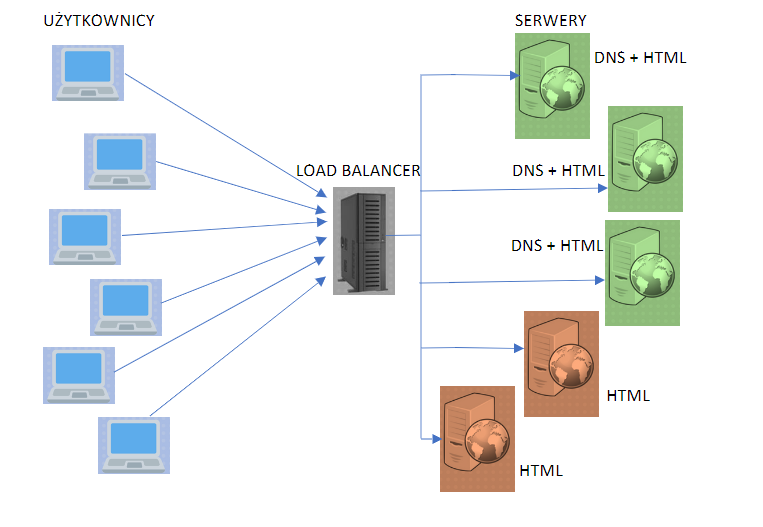
\includegraphics[width=\textwidth]{chart-exercise.png}
\end{figure}

\chapter*{Zadanie 1}

Należy wyznaczyć symulacyjnie zależność pomiędzy średnią liczba zapytań nadchodzących w czasie jednej milisekundy(L) i średnim czasem oczekiwania na przetworzenie zapytania przez serwer. Przedstawić tę zależność na wykresie.

\section*{Rozwiązanie}

W ramach rozwiązaniu przygotowano kod symulujacy load balancer w języku R przy użyciu pakietu simmer.

Symulacja używa dwóch obiektów trajektorii, jednego dla zapytań DNS, który kierowany jest do serwerów obsługujących zapytania DNS. Druga natomiast reprezentuje zapytania HTML i kierowana jest do serwerów HTML.

Czas przetwarzania zapytań opisany jest przez dwa parametry.
\begin{itemize}
  \item M - średni czas przetwarzania zapytania w milisekundach.
  \item SD - Odchylenie standardowe czasu przetwarzania zapytań.
\end{itemize}

Dla zapytań DNS przyjęto wartosć parametru M jako wartość 10 i użyto oznaczenia M1. Wartość parametru SD wynosi natomiast 2, a oznaczenie w kodzie to SD1.

W przypadku zapytań HTML, parametr M wynosi 20 i oznaczone jest przez M2, parametr SD wynosi również 2 i oznaczony jest jako SD2.

W ramach zadania load balancer kieruje zapytania do serwera z najmniejszą kolejką, parametr lb\_policy o wartości "shortest\_queue".

Ponadto zgodnie z założeniami połowa zapytań to zapytania DNS, druga połowa to zapytania HTML. Na końcu kod oblicza średni czas oczekiwania dla poszczególnych zapytań.

\newpage

\begin{verbatim}
  dns <- trajectory("dns_path") %>%
    select("dns_html", policy = lb_policy) %>% 
    seize_selected() %>%
    timeout(function() rnorm(1, M1, SD1)) %>%
    release_selected()

  html <- trajectory("html_path") %>%
    select(c("dns_html", "html"), policy = lb_policy) %>%
    seize_selected() %>%
    timeout(function() rnorm(1, M2, SD2)) %>%
    release_selected()

  envs <- mclapply(L_values, function(q) {
    simmer("servers") %>%
      add_resource("dns_html", 3) %>%
      add_resource("html", 2) %>%
      add_generator("dns", dns, function() rexp(1, q) * 2) %>%
      add_generator("html", html, function() rexp(1, q) * 2) %>%
      run(10000) %>%
      wrap()
  }, mc.cores = parallel::detectCores())

  results <- get_mon_arrivals(envs) %>% 
    transform(waiting_time = end_time - start_time - activity_time)

  mean_waiting_time <- c()
  for (i in 1:max(results$replication)){
    mean_waiting_time[i] <- mean(
      results$waiting_time[results$replication == i]
    )
  }
\end{verbatim}

\section*{Wyniki}

Jak widać na poniższym wykresie kolejka zaczyna się tworzyć przy relatywnie niewielkiej ilości zapytań na milisekundę.

\begin{figure}[H]
  \centering
  \includegraphics*[width=\textwidth]{image.png}
\end{figure}

\section*{Wnioski}

Przyjęte parametry opisujące czasu przetwarzania zapytań powoduja występowanie kolejek już dla stosunkowo małej liczby zapytań, nie bez znaczenia jednak pozostaje czas w jakim te zapytania nadchodzą.

Ponadto, nawet jeśli sam load balancer nie przetwarza zapytań ich przekierowanie zajmuje pewien czas co ogranicza przepustowosć całego modelu. To zaś ma odwzorowanie w czasie oczekiwania dla zapytań.

\chapter*{Zadanie 2}

O ile procent wzrośnie średni czas oczekiwania na przetworzenie zapytania gdy awarii ulegnie:
\begin{itemize}
  \item Jeden serwer HTML?
  \item Dwa serwery HMTL+DNS?
  \item load balancer (będzie kierował zapytania do losowo wybranego serwera zamiast do serwera z najkrótszą kolejką oczekujących zapytań)
\end{itemize}

\section*{Rozwiązanie}

Sama symulacja realizowana jest w sposób analogiczny do kodu z zadania nr 1.

\begin{small}
\begin{verbatim}
  library(simmer)
  library(parallel)
  
  set.seed(42)
  
  M1 <- 10 # Średni czas przetwarzania zapytań DNS
  SD1 <- 2 #Odchylenie standardowe czasu przetwarzania zapytań DNS
  M2 <- 20 # Średni czas przetwarzania zapytań HTML
  SD2 <- 2 #Odchylenie standardowe czasu przetwarzania zapytań HTML
  L_values <- seq(0.1, 0.5, 0.01)
  
  run_simulation <- function(num_dns_html, num_html, lb_policy) {
  
    dns <- trajectory("dns_path") %>%
      select("dns_html", policy = lb_policy) %>% 
      seize_selected() %>%
      timeout(function() rnorm(1, M1, SD1)) %>%
      release_selected()
  
    html <- trajectory("html_path") %>%
      select(c("dns_html", "html"), policy = lb_policy) %>%
      seize_selected() %>%
      timeout(function() rnorm(1, M2, SD2)) %>%
      release_selected()
  
    envs <- mclapply(L_values, function(q) {
      simmer("servers") %>%
        add_resource("dns_html", num_dns_html) %>%
        add_resource("html", num_html) %>%
        add_generator("dns", dns, function() rexp(1, q) * 2) %>%
        add_generator("html", html, function() rexp(1, q) * 2) %>%
        run(10000) %>%
        wrap()
    }, mc.cores = parallel::detectCores())
  
    results <- get_mon_arrivals(envs) %>% 
      transform(waiting_time = end_time - start_time - activity_time)
  
    mean_waiting_time <- c()
    for (i in 1:max(results$replication)){
      mean_waiting_time[i] <- mean(
        results$waiting_time[results$replication == i]
      )
    }
  
    return(mean_waiting_time)
  }
  
  original_waiting_time_vector <- run_simulation(3, 2, "shortest-queue")
  original_waiting_time <- mean(original_waiting_time_vector)
  
  one_html_failed_waiting_time <- mean(
    run_simulation(3, 1, "shortest-queue")
    )
  two_dns_html_failed_waiting_time <- mean(
    run_simulation(1, 2, "shortest-queue")
    )
  random_lb_waiting_time <- mean(run_simulation(3, 2, "random"))
  
  percentage_increase_one_html_failed <- (
    (
      one_html_failed_waiting_time - original_waiting_time
    ) / original_waiting_time
  ) * 100
  
  percentage_increase_two_dns_html_failed <- (
    (
      two_dns_html_failed_waiting_time - original_waiting_time
    ) / original_waiting_time
  ) * 100
  
  percentage_increase_random_lb <- (
    (random_lb_waiting_time - original_waiting_time) / original_waiting_time
  ) * 100
  
  cat("Percentage increase with one HTML server failure:", 
      percentage_increase_one_html_failed, "%\n")
  cat("Percentage increase with two DNS+HTML server failures:", 
      percentage_increase_two_dns_html_failed, "%\n")
  cat("Percentage increase with random load balancer:",
   percentage_increase_random_lb, "%\n")
  
  plot(L_values, original_waiting_time_vector, type="l", col="red",
        xlab="L (average requests per millisecond)", 
        ylab="mean waiting time [seconds]")
\end{verbatim}
\end{small}

Główna różnica polega na dodaniu obliczeń związanych z obliczaniem wartości procentowego wzrostu czasu oczekiwania dla poszczególnych scenariuszy oraz opakowaniu kodu z zadania 1 w funkcje. Takie podejście pozwoliło na proste uruchamianie wielokrotnie symulacji bezp otrzeby powielania jej kodu.

\section*{Wyniki}

Dla przedstawionych sceneriuszy procentowy wzrost średniego czasu oczekiwania dla zapytań wynosi:
\begin{itemize}
  \item Awaria pojedynczego serwera HTML: 86.32795\%
  \item Awaria dwóch serwerów DNS+HTML: 311.8372\%
  \item Awaria load balancera: 28.23808\%
\end{itemize}

\section*{Wnioski}

Wyniki te odpowiadają spodziewanym rezultatom. Czas oczekiwania dla zapytań wzrósł znaczono przy awarii dwóch serwerów, których brach szczególnie dotkliwie oddziałowuje na zapytania DNS. Ponieważ w takiej sytuacji wszystkie zapytania DNS wysyłane są do jednego serwera, dla zapytań HTML pozostały de facto dwa z pięciu serwerów.

Tego problemu nie można zaobserwować przy awarii pojedynczego serwera HTML, ponieważ jego rolę przejmą pozostałe cztery.

Podobnie sprawa ma się przy awarii load balancera, który zamiast wybierać serwer z najkrótszą kolejką, będzie rozdzielał zapytania w sposób losowy. Nie ma to znaczącego wpływu na czas oczekiwania, ponieważ zapytania wciąż mają dużą szansę trafić na mniej obciążony serwer.

\end{document}